\chapter{Gaussian Processes}\label{sec:Gaussian_processes}

\vfill
\localtableofcontents
\vfill
\newpage

\section{Introduction}

The analytical and Monte Carlo methods of \cref{sec:Bayesian_estimation} all assume the observation function $h_k$ to be fully known. However, many navigation scenarios depend on a physical field that is either unavailable or known only through scarce and noisy measurements.

A first way to fill this gap is to reconstruct the field directly from the measurements: \textbf{TODO: j'avais oublié, mais à reprendre + présenter des cas d'application au krigeage}
\begin{itemize}
	\item Deterministic interpolation, through nearest-neighbour selection, multilinear interpolation over a regular grid, or spline fitting;
	\item Linear regression on a fixed basis, such as polynomials or sinusoids;
	\item More expressive models, such as neural networks.
\end{itemize}
All of them return a single value at the queried location, without quantifying how much it can be trusted. Their use in the filters of \cref{sec:Bayesian_estimation}, however, requires the observation likelihood $p(z_k|x_k)$, a full distribution rather than a point prediction. The reconstruction error must then be absorbed into the observation noise, usually as a covariance held constant over the whole domain, although this error is almost zero next to a measurement and grows in sparsely sampled regions.

This chapter instead models such fields as a Gaussian process (GP), an adaptable framework that encodes both a prior expectation of the field and its spatial correlation structure. Together with its uncertainty, the resulting estimator can then serve as a surrogate observation model \cite{bib:GP-BayesFilters,bib:SLAM-GP-terrain} for the filters of \cref{sec:Bayesian_estimation}.

The rest of this chapter is organised as follows:
\begin{itemize}
	\item\Cref{sec:GP_definition} defines GPs through their mean functions and covariance kernels. It discusses the choice of kernel.
	\item\Cref{sec:kriging} then introduces kriging as a map reconstruction tool in situations where we are given preexisting data samples.
	\item\Cref{sec:reduced_rank} addresses the cost of inverting large Gram matrices in kriging by approximating $k$ with a reduced-rank kernel, therefore lowering the effective complexity of kriging methods.
	\item Finally, \cref{sec:RKHS} derives two representations of the mean function over a dictionary of functions, used to reconstruct the field when no prior knowledge is available.
\end{itemize}

\section{Definition and Properties}\label{sec:GP_definition}

Formally, a stochastic process generalises the notion of random variable to a random function, \textit{i.e.} a family $(f(x))_{x\in\mathcal{U}}$ of random variables indexed by a set $\mathcal{U}$, which may represent time $\mathbb{R}_+$, physical space $\mathbb{R}^2$ or $\mathbb{R}^3$, or any other domain. As shown by \Cref{th:GP_definition}, a GP is a special case of stochastic process \cite{bib:random-fields}.

\begin{definition}[Gaussian process]\label{th:GP_definition}
	For $d_z\in\mathbb{N}^*$, a stochastic process $(f(x))_{x\in\mathcal{U}}$ taking values in $\mathbb{R}^{d_z}$ is a GP if every finite linear combination of its values follows a Gaussian distribution. Formally, for all $n\in\mathbb{N}^*$, all $x_1,\dots,x_n\in\mathcal{U}$ and all $a_1,\dots,a_n\in\mathbb{R}^{d_z}$, there exist $m\in\mathbb{R}^{d_z}$ and $P\in\mathcal{S}_{d_z}^+(\mathbb{R})$ such that:
	\begin{equation}
		\sum_{i=1}^na_i^\top f(x_i)\sim\mathcal{N}(m,P)
	\end{equation}

	The GP is said to be non-degenerate if $P\succ0$ whenever the $x_1,\dots,x_n$ are pairwise distinct and the coefficients $a_1,\dots,a_n$ are not all zero.
\end{definition}

A GP is associated with a mean function:
\begin{equation}
	m:\left\{\begin{aligned}
	\mathcal{U}&\to\mathbb{R}^{d_z}\\
	x&\mapsto\mathbb{E}[f(x)]
	\end{aligned}\right.
\end{equation}
and a covariance kernel:
\begin{equation}
	k:\left\{\begin{aligned}
	\mathcal{U}\times\mathcal{U}&\to\mathcal{M}_{d_z,d_z}(\mathbb{R})\\
	x,x'&\mapsto\mathbb{E}\left[(f(x)-m(x))(f(x')-m(x'))^\top\right]
	\end{aligned}\right.
\end{equation}

\subsection{Basic Properties}

As shown by \Cref{th:GP_marginals}, $m$ and $k$ entirely characterise every finite-dimensional marginal of $f$. By Kolmogorov's extension theorem, they also uniquely determine the law of $f$. We thus write $f\sim\mathcal{GP}(m,k)$ for a GP with mean function $m$ and covariance kernel $k$.

\begin{proposition}[Finite-dimensional marginals]\label{th:GP_marginals}
	For $n\in\mathbb{N}^*$, let $x_1,\dots,x_n$ be pairwise distinct elements of $\mathcal{U}$. The joint distribution of $F\triangleq\left[f(x_1)^\top,\dots,f(x_n)^\top\right]^\top$ is the multivariate Gaussian distribution:
	\begin{equation}
		\begin{bmatrix}
		f(x_1)\\\vdots\\f(x_n)
		\end{bmatrix}\sim\mathcal{N}\left(\begin{bmatrix}
		m(x_1)\\\vdots\\m(x_n)
		\end{bmatrix},\begin{bmatrix}
		k(x_1,x_1)&\cdots&k(x_1,x_n)\\\vdots&\ddots&\vdots\\k(x_n,x_1)&\cdots&k(x_n,x_n)
		\end{bmatrix}\right)\label{eq:GP_marginals}
	\end{equation}
	where each block $k(x_i,x_j)\in\mathcal{M}_{d_z,d_z}(\mathbb{R})$.
\end{proposition}

\begin{proof}
	According to \Cref{th:GP_definition}, every linear combination:
	\begin{equation}
		a^\top F=\sum_{i=1}^na_i^\top f(x_i),\qquad a\triangleq\begin{bmatrix}a_1\\\vdots\\a_n\end{bmatrix}\in\mathbb{R}^{nd_z}
	\end{equation}
	is Gaussian. By the Cramér-Wold theorem \cite{bib:Cramér-Wold} $F$ is thus also a Gaussian vector of $\mathbb{R}^{nd_z}$.

	Such a vector is entirely determined by its mean and covariance, which we compute. In particular, we have:
	\begin{equation}
		\mathbb{E}[F]=\begin{bmatrix}\mathbb{E}[f(x_1)]\\\vdots\\\mathbb{E}[f(x_n)]\end{bmatrix}=\begin{bmatrix}m(x_1)\\\vdots\\m(x_n)\end{bmatrix}
	\end{equation}

	By definition of $k$, it comes that:
	\begin{equation}
		\begin{aligned}
		\mathbb{V}[F]&=\begin{bmatrix}
		\mathbb{E}\left[(f(x_i)-m(x_i))(f(x_j)-m(x_j))^\top\right]
		\end{bmatrix}_{i,j=1}^n\\
		&=\begin{bmatrix}
		k(x_i,x_j)
		\end{bmatrix}_{i,j=1}^n
		\end{aligned}
	\end{equation}
	which is exactly \eqref{eq:GP_marginals}.
\end{proof}

For two tuples of inputs $\mathbf{x}\triangleq(x_1,\dots,x_n)\in\mathcal{U}^n$ and $\mathbf{x}'\triangleq(x'_1,\dots,x'_p)\in\mathcal{U}^p$ of sizes $n,p\in\mathbb{N}^*$, we introduce the following vectorised notation:
\begin{align}
	f(\mathbf{x})&\triangleq\begin{bmatrix}
	f(x_1)\\\vdots\\f(x_n)
	\end{bmatrix}\\
	m(\mathbf{x})&\triangleq\begin{bmatrix}
	m(x_1)\\\vdots\\m(x_n)
	\end{bmatrix}\\
	k(\mathbf{x},\mathbf{x}')&\triangleq\begin{bmatrix}
	k(x_1,x'_1)&\cdots&k(x_1,x'_p)\\\vdots&\ddots&\vdots\\k(x_n,x'_1)&\cdots&k(x_n,x'_p)
	\end{bmatrix}
\end{align}

Using these notations, \Cref{th:GP_marginals} reads compactly:
\begin{equation}
	\forall n\in\mathbb{N}^*,\:\forall\mathbf{x}\in\mathcal{U}^n\text{ pairwise distinct},\:f(\mathbf{x})\sim\mathcal{N}\left(m(\mathbf{x}),k(\mathbf{x},\mathbf{x})\right)
\end{equation}

A GP is thus a consistent generalisation of the multivariate Gaussian distribution to an infinite and potentially continuous index set. Both of its parameters admit a direct interpretation. The mean function $m$ encodes prior knowledge about the average behaviour of $f$, while the kernel $k$ captures the correlation structure. The diagonal blocks $k(x,x)$ represent the covariance of $f(x)$, while the off-diagonal blocks $k(x,x')$, for $x\neq x'$, describe the cross-covariance between $f(x)$ and $f(x')$.

In order for the GP to be non-degenerate, the matrix $k(\mathbf{x},\mathbf{x})$ must be SPD in the sense of \Cref{th:matrix_SPSD} for every finite tuple $\mathbf{x}$ of pairwise distinct inputs. \Cref{th:kernel_SPSD} recasts this as a condition on $k$ alone \cite{bib:Schoenberg}, and \Cref{th:kernel_gram_equivalence} proves the equivalence between the two.

\begin{definition}[Symmetric positive definite kernel]\label{th:kernel_SPSD}
	A kernel $k:\mathcal{U}\times\mathcal{U}\to\mathcal{M}_{d_z,d_z}(\mathbb{R})$ is symmetric positive semi-definite (SPSD) if it is:
	\begin{itemize}
		\item\textbf{Symmetric:}
		\begin{equation}
			\forall x,x'\in\mathcal{U},\:k(x',x)=k(x,x')^\top
		\end{equation}
		\item\textbf{Positive semi-definite:}
		\begin{equation}
			\begin{gathered}
			\forall n\in\mathbb{N}^*,\:\forall x_1,\dots,x_n\in\mathcal{U},\:\forall a_1,\dots,a_n\in\mathbb{R}^{d_z},\\
			\sum_{i=1}^n\sum_{j=1}^na_i^\top k(x_i,x_j)\:a_j\geq0
			\end{gathered}
		\end{equation}
	\end{itemize}

	If the inequality is strict for every choice of pairwise distinct points $x_1,\dots,x_n$ and coefficients $a_1,\dots,a_n$ not all zero, then $k$ is symmetric positive definite (SPD).
\end{definition}

\begin{proposition}[Definite kernel/matrix equivalence]\label{th:kernel_gram_equivalence}
	The following equivalences hold:
	\begin{itemize}
		\item $k:\mathcal{U}\times\mathcal{U}\to\mathcal{M}_{d_z,d_z}(\mathbb{R})$ is a SPSD kernel if and only if, for every $n\in\mathbb{N}^*$ and every $\mathbf{x}\in\mathcal{U}^n$, $k(\mathbf{x},\mathbf{x})\in\mathcal{M}_{nd_z,nd_z}(\mathbb{R})$ is a SPSD matrix.
		\item $k$ is a SPD kernel if and only if, for every such tuple $\mathbf{x}$ of pairwise distinct points, $k(\mathbf{x},\mathbf{x})$ is a SPD matrix.
	\end{itemize}
\end{proposition}

\begin{proof}
	See \cref{sec:proof_definite_kernels}.
\end{proof}

\begin{remark}[Necessity of distinct points]
	While pairwise distinctness does not intervene in the computation of the strict version above, it is necessary for the SPD condition to be satisfiable. Indeed, at coinciding inputs $x_1=x_2$, the choice $a_1=-a_2=1$, with the other coefficients set to zero, cancels the quadratic form for non-zero coefficients, so no kernel could be SPD.
\end{remark}

\begin{remark}[Non-diagonal blocks]
	While \Cref{th:kernel_gram_equivalence} equates the SPDness of $k$ with that of $k(\mathbf{x},\mathbf{x})$ at distinct points, it does not make the off-diagonal blocks $k(x,x')$ SPD themselves. For $x\neq x'$, these may be non-positive or even non-symmetric.
\end{remark}

Throughout the rest of this document, we assume that the covariance kernel $k$ is SPD and that the points of every collection $\mathbf{x}=(x_1,\dots,x_n)\in\mathcal{U}^n$ are pairwise distinct. This ensures that we only work with non-degenerate GPs.

\subsection{Common Kernels}\label{sec:covariance_kernels}

Assume in this section that $\mathcal{U}$ is a finite-dimensional normed vector space, \textit{i.e.} $\mathcal{U}=\mathbb{R}^{d_x}$ for some $d_x\in\mathbb{N}^*$, up to isomorphism. A natural way to build kernels on $\mathcal{U}$ is to let the correlation between the field values at two points $x,x'$ depend only on the distance $\|x-x'\|$ between them. Kernels of this form are called radial kernels \cite{bib:Stein-kriging}, and are formally defined by \Cref{th:radial_kernel}.

Since $f$ typically represents a physical field, observations tend to become less correlated as the distance between them increases. \Cref{th:Matérn} introduces a common family of radial kernels modelling this behaviour, called the Matérn kernels \cite{bib:Matérn}. \Cref{th:Matérn_properties} then establishes their continuity and SPDness.

\begin{definition}[Radial kernel]\label{th:radial_kernel}
	A kernel $k:\mathbb{R}^{d_x}\times\mathbb{R}^{d_x}\to\mathcal{M}_{d_z,d_z}(\mathbb{R})$ is radial if there exists a function $\kappa:\mathbb{R}_+\to\mathcal{M}_{d_z,d_z}(\mathbb{R})$ and a norm $\|\cdot\|$ on $\mathbb{R}^{d_x}$ such that:
	\begin{equation}
		\forall x,x'\in\mathbb{R}^{d_x},\:k(x,x')=\kappa(\|x-x'\|)
	\end{equation}

	To simplify notations, we identify $\kappa$ with $k$ in the remainder of this document, such that we write:
	\begin{equation}
		\forall x,x'\in\mathbb{R}^{d_x},\:k(x,x')=k(\|x-x'\|)
	\end{equation}
\end{definition}

\begin{definition}[Matérn kernel]\label{th:Matérn}
	Assume that $d_z=1$, and let $\nu,l,\sigma_f^2\in\mathbb{R}_+^*$. The Matérn kernel of smoothness $\nu$, correlation length $l$, and characteristic variance $\sigma_f^2$ is the radial kernel defined as:
	\begin{equation}
		k_\nu:\left\{\begin{aligned}
		\mathbb{R}_+&\to\mathbb{R}_+\\
		r&\mapsto\sigma_f^2\:\frac{2^{1-\nu}}{\Gamma(\nu)}\left(\frac{\sqrt{2\nu}\:r}{l}\right)^\nu K_\nu\left(\frac{\sqrt{2\nu}\:r}{l}\right)
		\end{aligned}\right.
	\end{equation}
	where $\Gamma$ is the Gamma function, and $K_\nu$ is the modified Bessel function of the second kind \cite{bib:Abramowitz}.

	This family extends to $\nu=+\infty$ by taking the pointwise limit, yielding the squared exponential (SE) kernel:
	\begin{equation}
		k_{\mathrm{SE}}\triangleq k_{+\infty}:\left\{\begin{aligned}
		\mathbb{R}_+&\to\mathbb{R}_+\\
		r&\mapsto\sigma_f^2\:\exp\left(-\frac{r^2}{2\:l^2}\right)
		\end{aligned}\right.
	\end{equation}
\end{definition}

\begin{proposition}[Properties of Matérn kernels]\label{th:Matérn_properties}
	Let $\nu\in\mathbb{R}_+^*\cup\{+\infty\}$ and $l,\sigma_f^2\in\mathbb{R}_+^*$. The Matérn kernel associated with $\nu$, $l$ and $\sigma_f^2$ is a continuous SPD radial kernel.
\end{proposition}

\begin{proof}
	See \cref{sec:proof_Matérn}.
\end{proof}

The parameter $\nu$ controls the regularity. Indeed, for $p\in\mathbb{N}$, it can be shown \cite{bib:Rasmussen-covariance} that a GP equipped with $k_\nu$ is $p$ times mean-square differentiable if and only if $\nu>p$. For half-integer $\nu=p+\tfrac{1}{2}$, Matérn kernels can be written as the product of an exponential and a polynomial function of degree $p$:
\begin{equation}
	k_{p+1/2}(r)=\sigma_f^2\:\exp\left(-\frac{\sqrt{2p+1}r}{l}\right)\frac{\Gamma(p+1)}{\Gamma(2p+1)}\:\sum_{i=0}^p\frac{(p+i)!}{i!(p-i)!}\left(\frac{2\sqrt{2p+1}r}{l}\right)^{p-i}
\end{equation}

In particular, the following kernels correspond to usual choices of $\nu$, the SE kernel being recalled here for comparison:
\begin{itemize}
	\item\textbf{Exponential kernel.}
	\begin{equation}
		k_{1/2}(r)=\sigma_f^2\:\exp\left(-\frac{r}{l}\right)
	\end{equation}
	\item\textbf{Once-differentiable Matérn kernel.}
	\begin{equation}
		k_{3/2}(r)=\sigma_f^2\left(1+\frac{\sqrt{3}\:r}{l}\right)\exp\left(-\frac{\sqrt{3}\:r}{l}\right)
	\end{equation}
	\item\textbf{Twice-differentiable Matérn kernel.}
	\begin{equation}
		k_{5/2}(r)=\sigma_f^2\left(1+\frac{\sqrt{5}\:r}{l}+\frac{5\:r^2}{3\:l^2}\right)\exp\left(-\frac{\sqrt{5}\:r}{l}\right)
	\end{equation}
	\item\textbf{Squared exponential kernel.}
	\begin{equation}
		k_{+\infty}(r)=\sigma_f^2\:\exp\left(-\frac{r^2}{2\:l^2}\right)
	\end{equation}
\end{itemize}

\Cref{fig:Matérn} illustrates the radial decay of these kernels, evaluated with unit variance $\sigma_f^2=1$ and correlation length $l=1$ to facilitate comparison.

\begin{figure}[H]
	\centering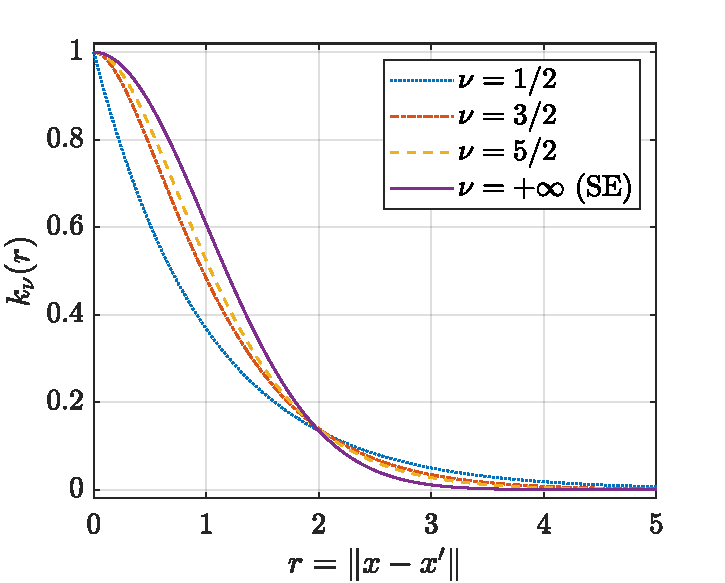
\includegraphics[width=0.7\textwidth]{../../Images/Noyaux de Matérn.pdf}
	\caption{Radial profile of Matérn kernels with increasing smoothness, together with their squared exponential limit. Larger values of $\nu$ produce smoother kernels, with flatter behaviours near the origin and faster-decaying tails.}\label{fig:Matérn}
\end{figure}

\begin{remark}[Anisotropic kernel]
	The norm used in \Cref{th:radial_kernel} does not necessarily need to be the canonical norm of $\mathbb{R}^{d_x}$. In particular, for $M\in\mathcal{S}_{d_x}^{++}(\mathbb{R})$, the Mahalanobis norm:
	\begin{equation}
		x\in\mathbb{R}^{d_x}\mapsto\|x\|_M\triangleq\sqrt{x^\top M^{-1}x}
	\end{equation}
	may produce anisotropic radial kernels in situations where $M$ is not proportional to the identity matrix.
\end{remark}

The main limitation of Matérn kernels is that they are scalar, while our observation model takes values in $\mathbb{R}^{d_z}$. To alleviate this issue, \Cref{th:separable_kernel} presents a method to create a vector-valued kernel from a scalar one.

\begin{proposition}[Separable kernel]\label{th:separable_kernel}
	Let $k:\mathcal{U}\times\mathcal{U}\to\mathbb{R}$ be a scalar SPD kernel, and let $\Sigma\in\mathcal{S}_{d_z}^{++}(\mathbb{R})$. Then:
	\begin{equation}
		k_{\mathrm{sep}}:\left\{\begin{aligned}
		\mathcal{U}\times\mathcal{U}&\to\mathcal{M}_{d_z,d_z}(\mathbb{R})\\
		x,x'&\mapsto\Sigma\:k(x,x')
		\end{aligned}\right.
	\end{equation}
	is a valid SPD kernel for an $\mathbb{R}^{d_z}$-valued GP.

	Furthermore, when $k$ is continuous, $k_{\mathrm{sep}}$ is also continuous.
\end{proposition}

\begin{proof}
	The symmetry and potential continuity of $k_{\mathrm{sep}}$ are direct from that of $k$ and $\Sigma$. The positive definiteness can be established by letting $A$ be a Cholesky factor of the SPD matrix $\Sigma$, and considering, for every $n\in\mathbb{N}^*$ and every not all zero coefficients $a_1,\dots,a_n\in\mathbb{R}^{d_z}$:
	\begin{equation}
		\forall i\in[\![1,n]\!],\:b_i\triangleq A^\top a_i
	\end{equation}

	Since $A$ is invertible, these coefficients are not all zero, and thus:
	\begin{equation}
		\begin{aligned}
		\sum_{i=1}^n\sum_{j=1}^na_i^\top k_{\mathrm{sep}}(x_i,x_j)\:a_j&=\sum_{i=1}^n\sum_{j=1}^na_i^\top A\:A^\top a_j\:k(x_i,x_j)\\
		&=\sum_{i=1}^n\sum_{j=1}^nb_i^\top b_j\:k(x_i,x_j)\\
		&=\sum_{l=1}^{d_z}\sum_{i=1}^n\sum_{j=1}^nb_i^{(l)}\:b_j^{(l)}\:k(x_i,x_j)
		\end{aligned}
	\end{equation}
	where $b_i^{(l)}$ denotes the $l$-th component of $b_i$. Each inner double sum is a quadratic form of $k$, hence non-negative, and at least one of them is strictly positive since at least one of the vectors $\left(b_1^{(l)},\dots,b_n^{(l)}\right)$ is non-zero.
\end{proof}

\begin{remark}[Multi-scale kernels]
	For $n\in\mathbb{N}^*$, $\Sigma_1,\dots,\Sigma_n\in\mathcal{S}_{d_z}^{++}(\mathbb{R})$ and $k^{(1)},\dots,k^{(n)}$ Matérn kernels of correlation lengths $l_1<\cdots<l_n\in\mathbb{R}_+^*$, the multi-scale kernel is:
	\begin{equation}
		k_{\mathrm{MS}}:\left\{\begin{aligned}
		\mathbb{R}_+&\to\mathcal{M}_{d_z,d_z}(\mathbb{R})\\
		r&\mapsto\sum_{i=1}^n\Sigma_i\:k^{(i)}(r)
		\end{aligned}\right.
	\end{equation}
	Each of its terms is separable in the sense of \Cref{th:separable_kernel}, hence SPD, and a sum of SPD kernels with positive coefficients is itself SPD. When the correlation lengths have different orders of magnitude, such kernels can be used to capture local fluctuations and global trends simultaneously.
\end{remark}

Every kernel considered in this section is specified by a set of hyperparameters, such as $\nu$, $l$ and $\sigma_f^2$ for a Matérn kernel, $\Sigma$ for its separable extension, or one such set per scale for a multi-scale model. Their estimation is a standard step in GP modelling, and is independent of bayesian estimation considerations. However, the specific characteristics of our applications can be used to improve the estimation of such hyperparameters. These aspects are thus discussed in \cref{sec:HP_estimation}, and the hyperparameters are assumed to be fully specified for the rest of this chapter.
